Dans ce chapitre nous présentons \langname, un langage impératif inspiré de C.
Sa syntaxe est tout d'abord décrite ; puis une sémantique opérationnelle est
explicitée.

Ce langage servira de support au systèmes de types décrit dans le
chapitre~\ref{cha:typbase} et enrichi dans le chapitre~\ref{cha:qualifs}.

La traduction depuis C sera explicitée dans le chapitre~\ref{cha:implem}.

\section{Notations}

\subsection*{Ensembles inductifs}

Dans ce chapitre (et les chapitres suivants), on définit de nombreux ensembles
inductifs. Plutôt que d'écrire la construction explicite par point fixe, on
emploie une notation en grammaire.

Étudions l'exemple des listes chaînées composées d'élements de $ℕ$.

Notons $L$ cet ensemble ; si $[]$ est la liste vide et $n::l$ la liste formée
d'une ``tête'' $n ∈ ℕ$ et d'une ``queue'' $l ∈ L$. Toute liste est donc d'une des
formes suivantes :

\begin{itemize}
\item $[]$
\item $n_1::[]$
\item $n_1::n_2::[]$
\item etc.
\end{itemize}

On peut donc $L$ de la manière inductive suivante :

\def\opfix{\textrm{fix}\xspace}

\begin{align*}
  \textsc{L} & = \opfix (L') \\
  L'(E) & = \{[]\} \cup \{ n::l / n ∈ ℕ, l ∈ E \} \\
\end{align*}

où

\begin{align*}
  \opfix (f) & = \bigcup_{n=0}^{\infty} f^{n}(∅) \\
  f^0(x) & = x \\
  ∀ n > 0, f^n(x) & = f^{n-1}(f (x)) \\
\end{align*}

(L'itération $n$ de l'union correspond aux listes comprenant au plus $n$
éléments)

Plutôt que d'écrire cette définition précise mais chargée, on écrira à la place
une définition en compréhension :

\gramlr{Listes}{
\begin{align*}
  l \gramisa & []   & \textrm{Liste vide}
  \\ \gramor & n::l & \textrm{Construction de liste}
\end{align*}
}

Chaque ensemble est identifié de manière unique par les noms de variables
métasyntaxiques : $n$ pour les entiers et $l$ pour les listes ici. Si plusieurs
métavariables du même ensemble doivent apparaître, elles sont indicées. Par
exemple, on peut définir des arbres binaires d'entiers de la manière suivante :

\gramlr{Arbres binaires}{
\begin{align*}
  a \gramisa & \textsc{F}           & \textrm{Feuille}
  \\ \gramor & \textsc{N}(a_1, n, a_2) & \textrm{Nœud}
\end{align*}
}

Cette notation a aussi l'avantage de s'étendre facilement aux définitions
mutuellement récursives.

\subsection*{Inférence}

La sémantique opérationnelle consiste en la définition d'une relation de
transition $\cdot\rightarrow\cdot$ entre états de l'interpréteur\footnote{Dans le
chapitre~\ref{cha:typbase}, la relation de typage $\cdot ⊢ \cdot : \cdot$ sera
définie par la même technique.}.

Cette relation est définie inductivement sur la syntaxe du programme. Plutôt que
de présenter l'induction explicitement, elle est représentée par des jugements
logiques et des règles d'inférences, de la forme :

\[
\irule{Nom}{P_1 \\ … \\ P_n}{C}
\]

Les $P_i$ sont les prémisses, et $C$ la conclusion. Cette règle s'interprète de
la manière suivante : si les $P_i$ sont prouvées, alors $C$ est prouvée.

Certaines règles n'ont pas de prémisse, ce sont des axiomes :

\[
\iaxiom{Ax}{A}
\]

Compte-tenu de la structure des règles, la preuve d'un jugement pourra donc être
vue sous la forme d'un arbre :

\[
  \irule{r1}{
    \irule{r2}
          {
            \iaxiom{r3}{A_1}
              \\
            \iaxiom{r4}{A_2}
          }
          {B_1}
    \\
    \irule{r5}
      {
        \iaxiom{r6} {A_3}
      }{B_2}
      }{C}
\]

\subsection*{Lentilles}

La notion d'accesseur utilisée ici est directement inspirée des \emph{lentilles}
utilisées en programmation fonctionnelle, décrite dans~\cite{PierceLenses}
et~\cite{LaarhovenLenses}.

\begin{definition}[Lentille]

Étant donnés deux ensembles $R$ et $A$, une \emph{lentille} $ℒ ∈
\setLens{R}{A}$ (ou \emph{accesseur}) est consistuée des opérations suivantes :

\begin{itemize}
\item
  une fonction de lecture $\mathrm{get}_ℒ : R → A$
\item
  une fonction de mise à jour $\mathrm{put}_ℒ : (A × R) → R$
\end{itemize}

telles que pour tous $a∈A, a'∈A, r∈R$ :

\begin{align*}
\tag{GetPut}
\mathrm{put}_ℒ(\mathrm{get}_ℒ(r), r) = & r \\
\tag{PutGet}
\mathrm{get}_ℒ(\mathrm{put}_ℒ(a, r)) = & a \\
\tag{PutPut}
\mathrm{put}_ℒ(a', \mathrm{put}_ℒ(a, r)) = & \mathrm{put}_ℒ(a', r) \\
\end{align*}

On note $ℒ =
\mkLens{\mathrm{get}_{ℒ}}{\mathrm{put}_{ℒ}}$.

\textsc{GetPut} signifie que si on lit une valeur puis qu'on la réecrit, l'objet
n'est pas modifié ; \textsc{PutGet} décrit l'opération inverse : si on écrit
une valeur dans le champ, c'est la valeur qui sera lue ; enfin, \textsc{PutPut}
évoque le fait que chaque écriture est totale : quand deux écritures se suivent,
seule la seconde compte.

\end{definition}

\begin{example}[Lentilles de tête et de queue de liste]

Soit $E$ un ensemble. On considère $L(E)$, l'ensemble des listes d'éléments de
$E$.

On définit les fonctions suivantes. Notons qu'elles ne sont pas définies sur la
liste vide $[]$, qui pourra être traité comme un cas d'erreur.

\begin{align*}
  \mathrm{get}_T     (t::q) = & t \\
  \mathrm{put}_T (t', t::q) = & t'::q \\
  \mathrm{get}_Q     (t::q) = & q \\
  \mathrm{put}_Q (q', t::q) = & t::q' \\
\end{align*}

Alors
$T = \mkLens{\mathrm{get}_T}{\mathrm{put}_T} ∈ \setLens{L(E)}{E}$
et
$Q = \mkLens{\mathrm{get}_Q}{\mathrm{put}_Q} ∈ \setLens{L(E)}{L(E)}$.

On a par exemple :

$\mathrm{get}_T (1::6::1::8::[]) = 1$

et :

$\mathrm{put}_Q (7, 3::6::1::5::[]) = 7::6::1::5::[]$.

\end{example}

\begin{proof}%{{{

Prouvons les trois propriétés pour $T$ et $Q$. En ignorant les cas d'erreur, on
peut toujours écrire une liste $l ∈ L(E)$ avec la forme $t::q$.

\paragraph{GetPut pour $T$}%{{{

\begin{align*}
\lensPut{T}{\lensGet{T}{l}}{l} & = \lensPut{T}{\lensGet{T}{t::q}}{t::q} \\
                               & = \lensPut{T}{t}{t::q} \\
                               & = t::q \\
                               & = l \\
\end{align*}%}}}

\paragraph{PutGet pour $T$}%{{{

\begin{align*}
\lensGet{T}{\lensPut{T}{a}{l}} & = \lensGet{T}{\lensPut{T}{a}{t::q}} \\
                               & = \lensGet{T}{a::q} \\
                               & = a \\
\end{align*}%}}}

\paragraph{PutPut pour $T$}%{{{

\begin{align*}
\lensPut{T}{a'}{\lensPut{T}{a}{l}} & = \lensPut{T}{a'}{\lensPut{T}{a}{t::q}} \\
                                   & = \lensPut{T}{a'}{a::q} \\
                                   & = a'::q \\
                                   & = \lensPut{T}{a'}{t::q} \\
                                   & = \lensPut{T}{a'}{l} \\
\end{align*}%}}}

\paragraph{GetPut pour $Q$}%{{{

\begin{align*}
\lensPut{Q}{\lensGet{Q}{l}}{l} & = \lensPut{Q}{\lensGet{Q}{t::q}}{t::q} \\
                               & = \lensPut{Q}{q}{t::q} \\
                               & = t::q \\
                               & = l \\
\end{align*}%}}}

\paragraph{PutGet pour $Q$}%{{{

\begin{align*}
\lensGet{Q}{\lensPut{Q}{a}{l}} & = \lensGet{Q}{\lensPut{Q}{a}{t::q}} \\
                               & = \lensGet{Q}{t::a} \\
                               & = a \\
\end{align*}%}}}

\paragraph{PutPut pour $Q$}%{{{

\begin{align*}
\lensPut{Q}{a'}{\lensPut{Q}{a}{l}} & = \lensPut{Q}{a'}{\lensPut{Q}{a}{t::q}} \\
                                   & = \lensPut{Q}{a'}{t::a} \\
                                   & = t::a' \\
                                   & = \lensPut{Q}{a'}{t::q} \\
                                   & = \lensPut{Q}{a'}{l} \\
\end{align*}%}}}

\end{proof}%}}}

\begin{definition}[Lentille indexée]

Les objets de certains ensembles $R$ sont composés de plusieurs sous-objets
accessibles à travers un indice $i ∈ I$. Une lentille indexée est une fonction
$Δ$ qui associe à un indice $i$ une lentille entre $R$ et un de ses champs
$A_i$:

\[
  ∀ i ∈ I, ∃ A_i, Δ(i) ∈ \setLens{R}{A_i}
\]

On note alors :

\begin{align*}
r [ i ]_Δ \eqdef & \mathrm{get}_{Δ(i)}(r) \\
r [ i ← a ]_Δ \eqdef & \mathrm{put}_{Δ(i)}(a, r) \\
\end{align*}

\end{definition}

\begin{example}[Lentille "n\ieme élément d'un tuple"]

Soient $n ∈ ℕ$, et $n$ ensembles $E_1, …, E_n$.

Pour tout $i ∈ [1; n]$, on définit :

\begin{align*}
g_i((x_1, …, x_n)) = & x_i \\
p_i(y, (x_1, …, x_n)) = & (x_1, …, x_{i-1}, y, x_{i+1}, …, x_n)\\
\end{align*}

Définissons $T(i) = \mkLens{g_i}{p_i}$. Alors $T(i) ∈ \setLens{(E_1×…×E_n)}{E_i}$.

Donc $T$ est une lentille indexée, et on a par exemple :

\begin{align*}
(3,1,4,1,5) [2]_T = & \mathrm{get}_{T(2)} ((3, 1, 4, 1, 5)) \\
                  = & 1 \\
\\
(9,2,6,5,3) [3 ← 1]_T = & \mathrm{put}_{T(3)} (1, (9,2,6,5,3)) \\
                      = & (9,2,1,5,3)
\end{align*}
\end{example}

\begin{proof}%{{{
Soit $i ∈ [1; n]$. On montre que $T(i) ∈ \setLens{(E_1×…×E_n)}{E_i}$.


\paragraph{GetPut}%{{{

On note $r = (x_1,…,x_n)$.

\begin{align*}
\lensPut{T(i)}{\lensGet{T(i)}{r}}{r} = & \lensPut{T(i)}{\lensGet{T(i)}{ (x_1,…,x_n) }}{ (x_1,…,x_n) } \\
                                     = & \lensPut{T(i)}{x_i}{ (x_1,…,x_n) } \\
                                     = & (x_1,…,x_{i-1},x_i,x_{i+1},…,x_n) \\
                                     = & r \\
\end{align*}%}}}

\paragraph{PutGet}%{{{

\begin{align*}
\lensGet{T(i)}{\lensPut{T(i)}{a}{r}} = & \lensGet{T(i)}{\lensPut{T(i)}{a}{ (x_1,…,x_n) }}  \\
                                     = & \lensGet{T(i)}{(x_1,…,x_{i-1},a,x_{i+1},…,x_n)} \\
                                     = & a \\
\end{align*}%}}}

\paragraph{PutPut}%{{{

\begin{align*}
\lensPut{T(i)}{a'}{\lensPut{T(i)}{a}{r}} = & \lensPut{T(i)}{a'}{\lensPut{T(i)}{a}{(x_1,…,x_n)}}  \\
                                         = & \lensPut{T(i)}{a'}{ (x_1,…, x_{i-1}, a, x_{i+1}, …, x_n) } \\
                                         = & (x_1,…, x_{i-1}, a', x_{i+1}, …, x_n) \\
                                         = & \lensPut{T(i)}{a'}{ (x_1,…,x_n) } \\
                                         = & \lensPut{T(i)}{a'}{r} \\
\end{align*}%}}}

\end{proof}%}}}

\begin{definition}[Composition de lentilles]
  \label{def:lens-comp}

  Soient $ℒ_1 ∈ \setLens{A}{B}$ et $ℒ_2 ∈ \setLens{B}{C}$.

  La composition de $ℒ_1$ et $ℒ_2$ est la lentille
  $ℒ ∈ \setLens{A}{C}$ définie de la manière suivante:

  \begin{align*}
    \mathrm{get}_{ℒ} (r) =&
        \mathrm{get}_{ℒ_2}
        (\mathrm{get}_{ℒ_1} r) \\
    \mathrm{put}_{ℒ} (a, r) =&
        \mathrm{put}_{ℒ_1} (\mathrm{put}_{ℒ_2}
        (a, \mathrm{get}_{ℒ_1} r), r) \\
  \end{align*}

  On notera alors $ℒ = ℒ_1 \ggg ℒ_2$.

\end{definition}

\begin{proof}
Pour prouver que $ℒ_1 \ggg ℒ_2 ∈ \setLens{A}{C}$, il suffit de prouver les trois
propriétés caractéristiques.

\paragraph{GetPut}%{{{

\begin{align*}
& \lensPut{ℒ}{
    \lensGet{ℒ}{r}
    }{
      r
    } \\
= & \{ \textrm{définition de } \lensGetX{ℒ} \} \\
& \lensPut{ℒ}
    {
      \lensGet{ℒ_2}{
        \lensGet{ℒ_1}{r}
      }
    }
    { r } \\
= & \{ \textrm{définition de } \lensPutX{ℒ} \} \\
& \lensPut
    {ℒ_1}
    {
      \lensPut
        {ℒ_2}
        {
          \lensGet{ℒ_2}
            {
              \lensGet{ℒ_1}{r}
            }
        }
        { \lensGet
            {ℒ_1}
            {r}
        }
    }
    {r} \\
= & \{ \textrm{\textsc{GetPut} sur $ℒ_2$} \} \\
& \lensPut
    {ℒ_1}
    {
      \lensGet{ℒ_1}{r}
    }
    {r} \\
= & \{ \textrm{\textsc{GetPut} sur $ℒ_1$} \} \\
& r \\
\end{align*}%}}}

\paragraph{PutGet}%{{{

\begin{align*}
& \lensGet{ℒ}
    {
      \lensPut{ℒ}
        {a}
        {r}
    } \\
= & \{ \textrm{définition de } \lensGetX{ℒ} \} \\
& \lensGet{ℒ_2}
    {
      \lensGet{ℒ_1}
        {
          \lensPut{ℒ}
            {a}
            {r}
        }
    } \\
= & \{ \textrm{définition de } \lensPutX{ℒ} \} \\
& \lensGet{ℒ_2}
    {
      \lensGet{ℒ_1}
        {
          \lensPut{ℒ_1}
            {
              \lensPut{ℒ_2}
                {a}
                { \lensGet{ℒ_1}{r} }
            }
            { r }
        }
    } \\
= & \{ \textrm{\textsc{PutGet} sur $ℒ_1$} \} \\
& \lensGet{ℒ_2}
    {
      \lensPut{ℒ_2}
        {a}
        { \lensGet{ℒ_1}{r} }
    } \\
= & \{ \textrm{\textsc{PutGet} sur $ℒ_2$} \} \\
& a \\
\end{align*}%}}}

\paragraph{PutPut}%{{{

\begin{align*}
& \lensPut{ℒ}{a'}{
    \lensPut{ℒ}{a}{r}
  } \\
= & \{ \textrm{définition de } \lensPutX{ℒ} \} \\
& \lensPut{ℒ}{a'}{
    \lensPut{ℒ_1}
      {
        \lensPut{ℒ_2}
          {a}
          { \lensGet{ℒ_1}{r} }
      }
      { r }
  } \\
= & \{ \textrm{définition de } \lensPutX{ℒ} \} \\
& \lensPut{ℒ_1}
    {
      \lensPut{ℒ_2}
        {a'}
        { \lensGet{ℒ_1}{
            \lensPut{ℒ_1}
              {
                \lensPut{ℒ_2}
                  {a}
                  { \lensGet{ℒ_1}{r} }
              }
              { r }
          }
        }
    }
    {
        \lensPut{ℒ_1}
          {
            \lensPut{ℒ_2}
              {a}
              { \lensGet{ℒ_1}{r} }
          }
          { r }
    } \\
= & \{ \textrm{\textsc{GetPut} sur $ℒ_1$} \} \\
& \lensPut{ℒ_1}
    {
      \lensPut{ℒ_2}
        {a'}
        {
          \lensPut{ℒ_2}
            {a}
            { \lensGet{ℒ_1}{r} }
        }
    }
    {
        \lensPut{ℒ_1}
          {
            \lensPut{ℒ_2}
              {a}
              { \lensGet{ℒ_1}{r} }
          }
          { r }
    } \\
= & \{ \textrm{\textsc{PutPut} sur $ℒ_2$} \} \\
& \lensPut{ℒ_1}
    {
      \lensPut{ℒ_2}
        {a'}
        { \lensGet{ℒ_1}{r} }
    }
    {
        \lensPut{ℒ_1}
          {
            \lensPut{ℒ_2}
              {a}
              { \lensGet{ℒ_1}{r} }
          }
          { r }
    } \\
= & \{ \textrm{\textsc{PutPut} sur $ℒ_1$} \} \\
& \lensPut{ℒ_1}
    {
      \lensPut{ℒ_2}
        {a'}
        { \lensGet{ℒ_1}{r} }
    }
    { r
    } \\
= & \{ \textrm{définition de } \ggg \} \\
& \lensPut{ℒ}{a'}{r} \\
\end{align*}%}}}

\end{proof}

\section{But et comparaison à C}

Le langage C~\cite{KandR} est un langage impératif, conçu pour être un
``assembleur portable''. Ses types de données et les opérations associées sont
donc naturellement très bas niveau.

Les types de données de C sont établis pour représenter les mots mémoire
manipulables par les processeurs : essentiellement des entiers et flottants de
plusieurs tailles. Les types composés correespondent à des zones de mémoire
contigües, homogènes (dans le cas des tableaux) ou hétérogènes (dans le cas des
structures).

Une des spécificités de C est qu'il expose au programmeur la notion de pointeur,
c'est à dire des variables qui représentent directement une adresse en mémoire.
Les pointeurs peuvent être typés (on garde une indication sur le type de l'objet
stocké à cette adresse) ou non typés.

Le système de types rudimentaire de C ne permet pas d'avoir beaucoup de
garanties sur la sûreté du programme. En effet, aucune vérification n'est
effectuée en dehors de celles faites par le programmeur.

Le but ici est d'établir un langage plus simple mais qui permettra de raisonner
sur une certaine classe de programmes C.

\section{Principes}

Nous voulons capturer l'essence de C. Les traits principaux sont les suivants :

\paragraph{Types de données :} très simples. Entiers machine, flottants,
pointeurs et types composés (structures et tableaux) composés de ceux-ci.

\paragraph{Variables :} elles sont mutables, et on peut passer des données par
valeur ou par pointeur.

\paragraph{Flôt de contrôle :} il repose sur les construction ``if'' et
``while''. Les autres types de boucle (``for'' et ``do/while'') peuvent être
construits avec ces opérateurs.

\paragraph{Fonctions :} le code est organisé en fonctions ``simples'',
c'est-à-dire qui ne sont pas des fermetures. Même si le corps
d'une fonction peut être inclus dans le corps d'une autre, il n'est pas possible
d'accéder aux variables de la portée entourante depuis la fonction intérieure.

\section{Syntaxe}

Les figures~\ref{fig:stx}, \ref{fig:stx-data} et \ref{fig:stx-ops} présentent
notre langage intermédiaire. Il contient la plupart des fonctionnalités
présentes dans les langages impératifs comme C.

%TODO ordre

Un programme est organisé en fonctions, qui contiennent des instructions, qui
elles-mêmes manipulent des expressions.

Le flot de contrôle est simplifié par rapport à C : il ne contient que
l'alternative ("if") et la boucle "while". Les autres formes de boucle
("do/while" et "for") peuvent être émulées par une boucle "while".

Les fonctionnalités manquantes, et comment les émuler, seront discutés dans le
chapitre~\ref{cha:conclusion}. % TODO vraiment ?

Pour l'alternative, on introduit également la forme courte $\iThen{e}{i} =
\iIf{e}{i}{\iPass}$.

Les opérateurs sont donnés dans la figure~\ref{fig:stx-ops}.

\begin{figure}

  \gramlr{Constantes}{
    \begin{align*}
      c \gramisa & i      & \textrm{Entier}
      \\ \gramor & d      & \textrm{Flottant}
      \\ \gramor & \eNull & \textrm{Pointeur nul}
    \end{align*}
  }

  \gramlr{Expressions}{
    \begin{align*}
      e \gramisa & c               & \textrm{Constante}
      \\ \gramor & lv              & \textrm{Accès mémoire}
      \\ \gramor & \opun~e         & \textrm{Opération unaire}
      \\ \gramor & e~\opbin~e      & \textrm{Opération binaire}
      \\ \gramor & \& lv           & \textrm{Pointeur}
      \\ \gramor & lv ← e          & \textrm{Affectation}
      \\ \gramor & \{ l_1 : e_1 ;
                  … ; l_n : e_n \} & \textrm{Structure}
      \\ \gramor & \{e_1 ;…; e_n\} & \textrm{Tableau}
      \\ \gramor & f               & \textrm{Fonction}
      \\ \gramor & e (e_1, …, e_n) & \textrm{Appel de fonction}
    \end{align*}
  }

  \gramlr{Left-values}{
    \begin{align*}
      lv \gramisa & x     & \textrm{Variable}
      \\  \gramor & *lv   & \textrm{Déréférencement}
      \\  \gramor & lv.l  & \textrm{Accès à un champ}
      \\  \gramor & lv[e] & \textrm{Accès à un élément}
    \end{align*}
  }
  \caption{Syntaxe - expressions}
  \label{fig:stx-data}
\end{figure}

\begin{figure}
  \gramlr{Instructions}{
    \begin{align*}
      i \gramisa & \iPass        & \textrm{Instruction vide}
      \\ \gramor & i;i           & \textrm{Séquence}
      \\ \gramor & e             & \textrm{Expression}
      \\ \gramor & \iIf{e}{i}{i} & \textrm{Alternative}
      \\ \gramor & \iWhile{e}{i} & \textrm{Boucle}
      \\ \gramor & \iReturn{e}   & \textrm{Retour de fonction}
    \end{align*}
  }

  \gramlr{Fonctions}{
    \begin{align*}
      f \gramisa & \mathrm{fun} (x_1, …, x_n)    & \textrm{Arguments} \\
                 & ((x'_1, e_1), …, (x'_p, e_p)) & \textrm{Variables locales} \\
                 & \{ i \}                       & \textrm{Corps} \\
    \end{align*}
  }

  \gramlr{Phrases}{
    \begin{align*}
      p \gramisa & x = e             & \textrm{Variable globale}
      \\ \gramor & e                 & \textrm{Évaluation d'expression}
      \\ \gramor & \tstruct{s}
                      \{ x_1 : t_1
                       ; …
                       ;  x_n : t_n
                      \}             & \textrm{Déclaration de structure}
    \end{align*}
  }

  \gramlr{Programme}{
    \begin{align*}
      P \gramisa & (p_1, …, p_n) & \textrm{Phrases}
    \end{align*}
  }

  \caption{Syntaxe - instructions}
  \label{fig:stx}
\end{figure}

\begin{figure}

  \gramlr{Opérateurs binaires}{
    \begin{align*}
      \opbin \gramisa & +,-,\times,/      & \textrm{Arithmétique entière}
      \\     \gramor  & +.,-.,\times.,/.  & \textrm{Arithmétique flottante}
      \\     \gramor  & +_p, -_p          & \textrm{Arithmétique de pointeurs}
      \\     \gramor  & =,≠,≤,≥,<,>       & \textrm{Comparaisons}
      \\     \gramor  & \&,|,\opxor       & \textrm{Opérateurs bit à bit}
      \\     \gramor  & \&\&,||           & \textrm{Opérateurs logiques}
      \\     \gramor  & \ll, \gg          & \textrm{Décalages}
    \end{align*}
  }

  \gramlr{Opérateurs unaires}{
    \begin{align*}
      \opun \gramisa & +,-   & \textrm{Arithmétique entière}
      \\    \gramor  & +.,-. & \textrm{Arithmétique flottante}
      \\    \gramor  & \sim  & \textrm{Négation bit à bit}
      \\    \gramor  & !     & \textrm{Négation logique}
    \end{align*}
  }

  \caption{Syntaxe - opérateurs}
  \label{fig:stx-ops}
\end{figure}

\section{Définitions préliminaires}

On suppose avoir à notre disposition un ensemble infini dénombrable
d'identificateurs \sId (par exemple des chaînes de caractères).

$X^*$ est l'ensemble des suites finies de $X$, indexées à partir de 1. Si $u ∈
X^*$, on note $|u|$ le nombre d'éléments de $u$ (le cardinal de son ensemble de
définition). Pour $1 ≤ i ≤ |u|$, on note $u_i = u(i)$ le i-ème élément de la
suite.

On peut aussi voir les suites comme des listes : on note $[]$ la suite vide,
telle que $|[]| = 0$. On définit en outre la construction de suite de la manière
suivante : si $x ∈ X$ et $u ∈ X^*$, la liste $x::u ∈ X^*$ est la liste $v$ telle
que :

\begin{align*}
  v_1 = & x \\
  ∀ i ∈ [1; |u|] , v_{i+1} = & u_i
\end{align*}

La concaténation des listes $u$ et $v$ est la liste $u@v = w$ telle que :

\begin{align*}
|w| = & |u| + |v| \\
∀ i ∈ [1 ; |u|] , w_i = & u_i \\
∀ j ∈ [1 ; |v|] , w_{|u| + j} = & v_j
\end{align*}

\section{Mémoire}

L'interprète que nous nous apprêtons à définir manipule des valeurs qui sont
associées aux variables du programme.

\begin{align*}
  \sVal = &          \sInt
            \bigdcup \sFloat
            \bigdcup \{ \eNull \}
            \bigdcup \sPhi \\
  \sInt = & ℤ/2^{32} ℤ - 2^{31} \\
  \sFloat = & \textsc{IeeeFloat}(32) \\
    \sPhi = & \mathrm{fix} (\sPhi') \\
    \sPhi'(X) = & X \\
                & \cup \sAddr \\
                & \cup \{*φ / φ ∈ \sPhi\} \\
                & \cup \{φ.c / φ ∈ \sPhi, c ∈ \sId\} \\
                & \cup \{φ[n] / φ ∈ \sPhi, n ∈ \sInt\} \\
  \sAddr = & \sId \bigdcup (ℕ × \sId) \\
\end{align*}

$\textsc{IeeeFloat}(n)$ correspond à l'ensemble des flottants IEEE 754 de $n$
bits\cite{ieee754}. Ici, \sInt est choisi pour représenter les nombres entiers
de $-2^{31}$ à $2^{31}-1$, mais ce choix est arbitraire : de la même manière, on
aurait pu choisir des nombres à 64 bits ou même de précision arbitraire.

L'ensemble des états mémoire est :

\[
  \sMem = ((\sId × \sVal)^*)^* × (\sId × \sVal)^*
\]

Un état mémoire état mémoire $(s, g) ∈ \sMem$ est composé :

\begin{itemize}
\item
  d'une part, d'une pile $s$ de cadres, qui sont des listes
  d'association (nom de variable, valeur).
\item
  d'autre part, une liste d'association qui représente les variables
  globales.
\end{itemize}

La structure de pile des locales permet de les organiser en niveaux indépendants:
à chaque appel de fonction, un nouveau cadre de pile est créé, comprenant ses
paramètres et ses variables locales.

Au contraire, pour les globales il n'y a pas de système d'empilement, puisque
ces variables sont accessibles depuis tout point du programme.

Ces définitions sont résumées dans la figure~\ref{fig:interp}. Plusieurs
constructions, comme les tableaux, sont ambigües puisqu'elle ont à la fois une
forme syntaxique et une forme sémantique. Pour lever cette ambigüité, on note
sous un accent circonflexe $\widehat{\cdot}$ les constructions syntaxique. Par
exemple, si $x$ vaut $2$ et $y$ vaut $3$, l'expression $\{ x, y \}$ s'évaluera
en valeur $\widehat{\{ 2, 3 \}}$


\begin{figure}

  \gramlr{Valeurs}{
    \begin{align*}
      v \gramisa & \widehat{c}     & \textrm{Constante}
      \\ \gramor & φ               & \textrm{Référence mémoire}
      \\ \gramor & \widehat{
                    \{ l_1 : v_1 ;
                  … ; l_n : v_n \}
                  }                & \textrm{Structure}
      \\ \gramor & \widehat{
                   \{v_1 ;…; v_n\}
                   }               & \textrm{Tableau}
      \\ \gramor & \widehat{f}     & \textrm{Fonction}
    \end{align*}
  }

  \gramlr{Adresses}{
    \begin{align*}
      a \gramisa & (n, x) & \textrm{Variable locale}
      \\ \gramor & x      & \textrm{Variable globale}
    \end{align*}
  }

  \gramlr{Chemins}{
    \begin{align*}
      φ \gramisa & a    & \textrm{Adresse}
      \\ \gramor & *φ   & \textrm{Déréférencement}
      \\ \gramor & φ.l  & \textrm{Accès à un champ}
      \\ \gramor & φ[n] & \textrm{Accès à un élément}
    \end{align*}
  }

  \gramlr{Pile}{
    \begin{align*}
      s \gramisa & []                       & \textrm{Pile vide}
      \\ \gramor & \{ x_1 ; … ; x_n \} :: s & \textrm{Ajout d'un cadre}
    \end{align*}
  }

  \gramlr{État mémoire}{
    \begin{align*}
      m \gramisa & (s,                    & \textrm{Pile}      \\
                 & \{ x_1 ;…; x_n \},     & \textrm{Globales}  \\
                 & \{a_1↦v_1;…;a_p↦v_p\}) & \textrm{Valeurs}
    \end{align*}
  }

  \caption{Composantes d'un état mémoire}
  \label{fig:interp}
\end{figure}

\begin{definition}[Recherche de variable]

  La recherche de variable permet d'associer à une variable $x$ une adresse $a$.

  Chaque fonction peut accéder aux variables locales de la fonction en cours,
  ainsi qu'aux variables globales.

  \begin{align*}
    \mathrm{Lookup} ((s, g), x) = & (|s|, x)
                                    \mbox{ si }|s| > 0
                                    \mbox{ et }∃ (x, v) ∈ s_1 \\
    \mathrm{Lookup} ((s, g), x) = & x \mbox{ si } (x, v) ∈ g
  \end{align*}

\end{definition}

En entrant dans une fonction, on rajoutera un cadre de pile qui contient les
paramètres de la fonction ainsi que ses variables locales. En retournant à
l'appelant, il faudra supprimer ce cadre de pile.

\begin{definition}[Manipulations de pile]

  On définit l'empilement d'un cadre de pile $c = ((x_1, v_1), …, (x_n, v_n))$
  sur un état mémoire $m = (s, g)$ (figure~\ref{fig:stackops-push}):

  \[
    \mathrm{Push}((s, g), c) = (c::s, g)
  \]

  On définit aussi l'extension du dernier cadre de pile
  (figure~\ref{fig:stackops-extend}):

  \[
    \mathrm{Extend}((c::s, g), x) = (((x @ c) :: s), g)
  \]

  De même on définit le dépilement (figure~\ref{fig:stackops-pop}):

  \[
    \mathrm{Pop}(c::s, g) = (s, g)
  \]

\end{definition}

\begin{figure}

  \centering

  \subfloat[Empilement]{
  \label{fig:stackops-push}
  \begin{tikzpicture}
    [ stack/.style={draw,shape=rectangle,minimum height=5mm,minimum width=2cm}
    , every node/.style={font=\footnotesize}
    , faded/.style={fill=black!20}
    ]


    \path (8,0)   node [stack, faded] {}
    -- ++ (0,0.5) node [stack, faded] {}
    -- ++ (0,0.5) node [stack, faded] {}
    ;

    \path (12,0)  node [stack, faded] {}
    -- ++ (0,0.5) node [stack, faded] {}
    -- ++ (0,0.5) node [stack, faded] {}
    -- ++ (0,0.5) node [stack] {$x↦0$}
    ;

    \draw [->] (9.2, 1) -- node[auto] {$\mathrm{Push}((x, 0))$} ++(1.6, 0);
  \end{tikzpicture}
  }

  \subfloat[Extension de cadre]{
  \label{fig:stackops-extend}

  \begin{tikzpicture}
    [ stack/.style={draw,shape=rectangle,minimum height=5mm,minimum width=2cm}
    , every node/.style={font=\footnotesize}
    , faded/.style={fill=black!20}
    ]


    \path (4,-3)  node [stack, faded] {}
    -- ++ (0,0.5) node [stack, faded] {}
    -- ++ (0,0.5) node [stack, faded] {}
    -- ++ (0,0.5) node [stack] {$x↦0$}
    ;

    \path (8,-3)  node [stack, faded] {}
    -- ++ (0,0.5) node [stack, faded] {}
    -- ++ (0,0.5) node [stack, faded] {}
    -- ++ (0,0.5) node [stack] {$x↦0, y↦3$}
    ;

    \draw [->] (5.2, -2) -- node[auto] {$\mathrm{Extend}((y, 3))$} ++(1.6, 0);

  \end{tikzpicture}
  }

  \subfloat[Dépilement]{
  \label{fig:stackops-pop}
  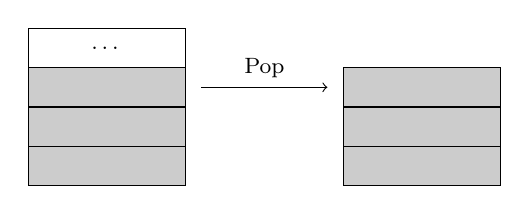
\begin{tikzpicture}
    [ stack/.style={draw,shape=rectangle,minimum height=5mm,minimum width=2cm}
    , every node/.style={font=\footnotesize}
    , faded/.style={fill=black!20}
    ]

    \path (0,0)   node [stack, faded] {}
    -- ++ (0,0.5) node [stack, faded] {}
    -- ++ (0,0.5) node [stack, faded] {}
    -- ++ (0,0.5) node [stack] {$…$}
    ;

    \path (4,0)   node [stack, faded] {}
    -- ++ (0,0.5) node [stack, faded] {}
    -- ++ (0,0.5) node [stack, faded] {}
    ;

    \draw [->] (1.2, 1) -- node[auto] {Pop} ++(1.6, 0);
  \end{tikzpicture}
  }

  \caption{Opérations de pile}
  \label{fig:stackops}
\end{figure}

\section{Accesseurs}

On définit ici quelques lentilles.

\begin{definition}[Accès à une liste d'associations]

  Une liste d'association est une liste de paires (clef, valeur) avec
  l'invariant supplémentaire que les clefs sont uniques. Il est donc possible de
  trouver au plus une valeur associée à une clef donnée. L'écriture est
  également possible, en remplaçant un couple par un couple avec une valeur
  différente.

  L'accesseur $[\cdot]_L$ est défini par :

  \begin{align*}
    l[x]_L     = & v \mbox{ où } \{v\} = \{y / (x, y) ∈ l\} \\
    l[x ← v]_L = & (x, v) :: \{ (y, v) ∈ g(x) / y ≠ x \})
  \end{align*}

\end{definition}

\begin{definition}[Accès par adresse]

  Les états mémoire sont constitués des listes d'association (nom, valeur).

  L'accesseur par adresse $[\cdot]_A$ permet de généraliser l'accès à ces
  valeurs en utilisant comme clef non pas un nom mais une adresse.

  Selon cette adresse, on accède soit à la liste des globales, soit à une des
  listes de la pile des locales.

  Pour $m = (s, g)$,

  \begin{align*}
    m [x]_A          = & g[x]_L           & \textrm{Lecture d'une globale} \\
    m [(n, x)]_A     = & s_{|l|-n+1}[x]_L & \textrm{Lecture d'une locale} \\
    m [x ← v]_A      = & (s, g[x←v]_L)    & \textrm{Écriture d'une globale} \\
    m [(n, x) ← v]_A = & (s', g)          & \textrm{Écriture d'une locale} \\
           \mbox{ où } & s'_{|l|-n+1} = s_{|l|-n+1}[x ← v]_L \\
                       & ∀ i ≠ |l|-n+1, s'_i = s_i
  \end{align*}

\end{definition}

Les numéros de cadre qui permettent d'identifier les globales (le $n$ dans $(n,
x)$) croissent avec la pile. D'autre part, l'empilement se fait en tête de liste
(près de l'indice 1). Donc pour accéder aux plus vieilles locales (numérotées
1), il faut accéder au dernier élément de la liste. Ceci explique pourquoi un
indice $|l|-n+1$ apparaît dans la définition précédente.

\begin{definition}[Accès par champ]

  Les valeurs qui sont des structures possèdent des sous-valeurs, associées à
  des noms de champ.

  L'accesseur $[ \cdot ]_L$ permet de lire et de modifier un champ de ces
  valeurs.

  C'est une erreur d'accéder à un champ d'une valeur non structure ($4[l]_L$ par
  exemple).

  \begin{align*}
    \{ l_1 : v_1; … ; l_n : v_n \}[l_i]_L = & v_i \\
    \{ l_1 : v_1; … ; l_n : v_n \}[l_p ← v]_L = & \{ l_1 : v'_1; … ; l_n : v'_n \} \\
          \mbox{ où } & v'_p = v \\
                      & ∀ i ≠ p, v'_i = v_i
  \end{align*}

\end{definition}

\begin{definition}[Accès par indice]

  On définit de même un accesseur $[\cdot]_I$ pour les accès par indice à des
  valeurs tableaux. Néanmoins le paramètre indice est toujours un entier et pas
  une expression arbitraire.

  \begin{align*}
    \{ v_1 ; … ; v_n \} [i]_I   = & e_i \\
    \{ v_1 ; … ; v_n \} [i←v]_I = & \{ v'_1 ; … ; v'_n \} \\
                      \mbox{ où } & v'_i = v \\
                                  & ∀j≠i, v'_j = v_j
  \end{align*}

\end{definition}

\begin{definition}[Accès par chemin]
  \label{def:acces-phi}

  L'accès par chemin $[\cdot]_Φ$ permet de lire et de modifier la mémoire en
  profondeur.

  On peut accéder directement à une variable:

  \begin{align*}
    Φ(a) = & A(a) \\
  \end{align*}

  Les accès à des sous-valeurs se font en composant les accesseurs
  (définition~\ref{def:lens-comp}) :

  \begin{align*}
    Φ(φ.l) = & Φ(φ) \ggg L(l) \\
    Φ(φ[i]) = & Φ(φ) \ggg I(i) \\
  \end{align*}

  Enfin, le déréférencement est défini comme suit :

  \begin{align*}
    m[*φ]_Φ       = & m[φ']_Φ \mbox{ où } φ' = m[φ]_Φ \\
    m[*φ ← v]_Φ   = & m[φ' ← v]_Φ \mbox{ où } φ' = m[φ]_Φ \\
  \end{align*}

\end{definition}

Cette dernière définition mérite une explication. Dans le cas de la lecture, il
suffit d'appliquer les bons accesseurs : $[\cdot]_L$ pour $φ.l$, etc.

En revanche, la modification est plus complexe. Les deux premiers cas ($φ = a$
et $φ = *φ'$) modifient directement une valeur complète (en modifiant une
association), mais les deux suivants ($φ = φ'.l$ et $φ = φ'[i]$) ne font
qu'altérer une sous-valeur existante. Il est donc nécessaire de procéder en 3
étapes :

\begin{itemize}
\item obtenir la valeur à modifier (soit $m[φ]_φ$)
\item construitre une valeur altérée (en appliquant par exemple $[l←v]_L$)
\item affecter cette valeur au même chemin (le $m[φ ← …]_φ$ externe)
\end{itemize}

Dans la suite, on notera uniquement $[\cdot]$ tous ces accesseurs lorsque ce
n'est pas ambigü.

\section{Contextes d'évaluation}

L'évaluation des expressions repose sur la notion de contextes d'évaluation.
L'idée est que si on peut évaluer une expression, alors on peut évaluer une
expression qui contient celle-ci.

Par exemple, supposons que $\mm{m}{f(3)}{m}{2}$. Alors on peut ajouter la
constante $1$ à gauche de chaque expression sans changer le résultat :
$\mm{m}{1+f(3)}{m}{1+2}$. On a utilisé le même contexte
$C = 1+\ctxEmpty$.

Pour pouvoir raisonner en termes de contextes, 3 points sont nécessaires :

\begin{itemize}
\item comment découper une expression selon un contextes
\item comment appliquer une règle d'évaluation sous un contexte
\item comment regrouper une expression et un contexte
\end{itemize}

\begin{figure}
\figctx{}

\caption{Contextes d'exécution}
\label{fig:eval-ctx}
\end{figure}

Le premier point consiste à définir les contextes eux-mêmes
(figure~\ref{fig:eval-ctx}).

Le deuxième est résolu les règles d'inférence suivantes :

\begin{mathpar}
  \semrule{Ctx}

  \semrule{Ctx-Lv}

  \semrule{Ctx-Instr}
\end{mathpar}

Enfin, le troisième revient à définit l'opérateur de substitution
$\phxx{\ctxSub}$ présent dans la règle précédente. Afin de pouvoir appliquer des
substitution au niveau des left-values et des instructions, on définit aussi
respectivement $\phxx{\ctxSubL}$ et $\phxx{\ctxSubI}$.

Dans la définition de l'ensemble des contextes, chaque cas hormis le cas de base
fait apparaître exactement un "$C$". Chaque contexte est donc constitué
d'exactement un "trou" $\ctxEmpty$ (une dérivation de $C$ est toujours
linéaire). L'opération de substitution consiste à remplacer ce trou, comme
décrit dans la figure~\ref{fig:ctx-sub}.

\begin{figure}
\begin{align*}
  \ctxSub{\ctxEmpty}{e_0} = & e_0 \\
  \ctxSub{(\ctxOp{C}{e}     )}{e_0} = & \ctxOp{\ctxSub{C}{e_0}}{e}      \\
  \ctxSub{(\ctxOp{v}{C}     )}{e_0} = & \ctxOp{v}{\ctxSub{C}{e_0}}      \\
  \ctxSub{(\ctxUnOp{C}      )}{e_0} = & \ctxUnOp{\ctxSub{C}{e_0}}       \\
  \ctxSub{(\ctxLvDeref{C}   )}{e_0} = & \ctxLvDeref{\ctxSub{C}{e_0}}    \\
  \ctxSub{(\ctxLvField{φ}{C})}{e_0} = & \ctxLvField{φ}{\ctxSub{C}{e_0}} \\
  \ctxSub{(\ctxLvIndex{φ}{C})}{e_0} = & \ctxLvIndex{φ}{\ctxSub{C}{e_0}} \\
  \ctxSub{(\ctxLvIndex{C}{e})}{e_0} = & \ctxLvIndex{\ctxSub{C}{e_0}}{e} \\
  \ctxSub{(\ctxSet{C}{e})    }{e_0} = & \ctxSet{\ctxSub{C}{e_0}}{e}     \\
  \ctxSub{(\ctxSet{φ}{C})    }{e_0} = & \ctxSet{φ}{\ctxSub{C}{e_0}}     \\
  \ctxSub{\{ l_1:v_1 ; …
     ; l_i:C ; … ; l_n:e_n \}}{e_0} = & \{ l_1:v_1 ; … ; l_i:\ctxSub{C}{e_0} ; … ; l_n:e_n \} \\
  \ctxSub{[ v_1 ; … ; C ; … ; e_n ]}{e_0} = & [ v_1 ; … ; \ctxSub{C}{e_0} ; … ; e_n ]    \\
  \ctxSub{C (e_1, …, e_n)          }{e_0} = & \ctxSub{C}{e_0} (e_1, …, e_n)              \\
  \ctxSub{f (v_1, …, C, …, e_n)    }{e_0} = & f (v_1, …, \ctxSub{C}{e_0}, …, e_n)        \\
  \\
  \ctxSub{(C;i              )}{e_0} = & \ctxSub{C}{e_0};i               \\
  \ctxSub{(\iIf{C}{i_1}{i_2})}{e_0} = & \iIf{\ctxSub{C}{e_0}}{i_1}{i_2} \\
  \ctxSub{(\iReturn{C}      )}{e_0} = & \iReturn{\ctxSub{C}{e_0}}       \\
\end{align*}

\begin{align*}
% C
\ctxSub{C_L}{e_0} = & \ctxSubL{C_L}{e_0} \\
\ctxSub{\ctxOp{C}{e}}{e_0} = & \ctxOp{\ctxSub{C}{e_0}}{e} \\
\ctxSub{\ctxOp{v}{C}}{e_0} = & \ctxOp{v}{\ctxSub{C}{e_0}} \\
\ctxSub{\ctxUnOp{C}}{e_0} = & \ctxUnOp{\ctxSub{C}{e_0}} \\
\ctxSub{\ctxSet{C}{e}}{e_0} = & \ctxSet{\ctxSub{C}{e_0}}{e} \\
\ctxSub{\ctxSet{φ}{C}}{e_0} = & \ctxSet{φ}{\ctxSub{C}{e_0}} \\
\ctxSub{\{ l_1:v_1 ; … ; l_i:C ; … ; l_n:e_n \}}{e_0} = & \{ l_1:v_1 ; … ; l_i:\ctxSub{C}{e_0} ; … ; l_n:e_n \} \\
\ctxSub{[ v_1 ; … ; C ; … ; e_n ]}{e_0} = & [ v_1 ; … ; \ctxSub{C}{e_0} ; … ; e_n ] \\
\ctxSub{C (e_1, …, e_n)}{e_0} = & \ctxSub{C}{e_0} (e_1, …, e_n) \\
\ctxSub{f (v_1, …, C, …, e_n)}{e_0} = & f (v_1, …, \ctxSub{C}{e_0}, …, e_n) \\
\\
% C_L
\ctxSubL{\ctxEmpty}{l_0} = & \ctxEmpty \\
\ctxSubL{\ctxLvDeref{C_L}}{l_0} = & \ctxLvDeref{\ctxSubL{C_L}{l_0}} \\
\ctxSubL{\ctxLvField{C_L}{l}}{l_0} = & \ctxLvField{\ctxSubL{C_L}{l_0}}{l} \\
\ctxSubL{\ctxLvIndex{C_L}{e}}{l_0} = & \ctxLvIndex{\ctxSubL{C_L}{l_0}}{e} \\
\ctxSub{\ctxLvIndex{φ}{C}}{e_0} = & \ctxLvIndex{φ}{\ctxSub{C}{e_0}} \\
\\
% % C_I
% \ctxSubI{C_I;i}{i_0} = & \ctxSubI{C_I}{i_0};i \\
%
% \iIf{C}{i_1}{i_2}
% \iReturn{C}
% C
\end{align*}

\caption{Substitution dans les contextes d'évaluation}
\label{fig:ctx-sub}
\end{figure}

Par exemple, décomposons l'évaluation de $e_1~\opbin~e_2$ en $v =
v_1~\widehat{\opbin}~v_2$ depuis un état mémoire $m$ (cf.
figure~\ref{fig:eval-ex-ctx}) :

\begin{enumerate}
\item
  on commence par évaluer, d'une manière ou d'une autre, l'expression
  $e_1$ en une valeur $v_1$. Le nouvel état mémoire est noté $m'$. Soit
  donc $\mm{m}{e_1}{m'}{v_1}$.
\item
  En appliquant la règle \textsc{Ctx} avec $C = \ctxOp{\ctxEmpty}{e_2}$ (qui est
  une des formes possibles pour un contexte d'évaluation), on déduit de 1. que
  $\mmstar{m}{e_1~\opbin~e_2}{m'}{v_1~\opbin~e_2}$
\item
  D'autre part, on évalue $e_2$ depuis $m'$. En supposant encore que
  l'évaluation converge, notons $v_2$ la valeur calculée et $m''$ l'état mémoire
  résultant : $\mm{m'}{e_2}{m''}{v_2}$.
\item
  Appliquons la règle~\textsc{Ctx} à 3. avec $C = \ctxOp{v_1}{\ctxEmpty}$. On
  obtient $\mmstar{m}{v_1~\opbin~e_2}{m'}{v_1~\opbin~v_2}$.
\item
  En combinant les résultats de 2. et 4. on en déduit que
  $\mmstar{m}{e_1~\opbin~e_2}{m''}{v_1\opbin~v_2}$.
% TODO comment combiner ?
\item D'après la règle~\textsc{Exp_Binop},
  $ \mmstar{m''}{v_1\opbin~v_2}{m''}{v_1~\widehat{\opbin}~v_2}$
\item D'après 5. et 6., on a par combinaison
  $\mmstar{m}{e_1~\opbin~e_2}{m''}{v}$
  en posant
  $v = v_1~\widehat{\opbin}~v_2$
  .
% TODO comment combiner ?
\end{enumerate}

\begin{figure} % {{{

\[
\inferrule*
  {
    \inferrule*[vdots=2em]
      {
        \inferrule*[right=(Ctx), leftskip=4cm, vdots=2em]
          {
            \mmstar{m}{e_1}{m'}{v_1}
            \\
            (C = \ctxOp{\ctxEmpty}{e_2})
          }
          {
            \mmstar{m}{e_1~\opbin~e_2}{m'}{v_1~\opbin~e_2}
          }
        \\
        \inferrule*[right=(Ctx), rightskip=4cm, vdots=2em]
          {
            \mmstar{m'}{e_2}{m''}{v_2}
            \\
            (C = \ctxOp{v_1}{\ctxEmpty})
          }
          {
            \mmstar{m}{v_1~\opbin~e_2}{m'}{v_1~\opbin~v_2}
          }
      }
      { \mmstar{m}{e}{m''}{v_1\opbin~v_2} }
    \\
    \inferrule*[right=(Exp-BinOp), rightskip=2cm, vdots=2em]
      { }
      { \mmstar{m''}{v_1\opbin~v_2}{m''}{v_1~\widehat{\opbin}~v_2} }
  }
  { \mmstar{m}{e}{m''}{v_1~\widehat{\opbin}~v_2} }
\]

\caption{Évaluation d'une expression}
\label{fig:eval-ex-ctx}

\end{figure} % }}}

\section{Expressions}

\begin{definition}[Évaluation d'une expression]

  L'évaluation d'une expression $e$ se fait sous un état mémoire particulier $m$
  et est susceptible de modifier celui-ci en le transformant en un nouveau $m'$.
  Le résultat est toujours une valeur $v$, c'est à dire que nous présentons pour
  les expressions une sémantique à grands pas. Cette évaluation est notée :

  \[
    \mm{m}{e}{m'}{v}
  \]

\end{definition}

\begin{definition}[Évaluation d'une left-value]

  L'évaluation d'une left-value $lv$ produit un "chemin" $φ$ dans une variable,
  qui est en fait équivalent à une left-value dont toutes les sous-expressions
  (d'indices) ont été évaluées.

  On note :

  \[
    \mmlv{m}{lv}{m'}{φ}
  \]

\end{definition}

La sémantique présentée n'a pas d'erreur explicite. Si aucune règle ne peut
s'appliquer, on considère que l'exécution est terminée.

Puisque des left-values peuvent apparaitre dans les expressions, et des
expressions dans les left-values (en indice de tableau), leurs règles
d'évaluation sont mutuellement récursives.

\subsection*{Left-values}

\begin{figure}

  \centering

  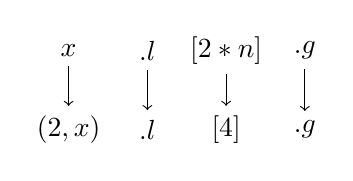
\begin{tikzpicture}
    \node              (a1) {$x$};
    \node[right of=a1] (a2) {$.l$};
    \node[right of=a2] (a3) {$[2*n]$};
    \node[right of=a3] (a4) {$.g$};

    \node[below of=a1] (b1) {$(2, x)$};
    \node[below of=a2] (b2) {$.l$};
    \node[below of=a3] (b3) {$[4]$};
    \node[below of=a4] (b4) {$.g$};

    \draw[->] (a1) -- (b1);
    \draw[->] (a2) -- (b2);
    \draw[->] (a3) -- (b3);
    \draw[->] (a4) -- (b4);
  \end{tikzpicture}

  \caption{Évaluation des left-values.}
  \label{fig:eval-lv}
\end{figure}

Obtenir un chemin à partir d'un nom de variable revient à résoudre le nom de
cette variable : est-elle accessible ? Le nom désigne-t'il une variable locale
ou une variable globale ?

\begin{mathpar}
  \semrule{Phi-Var}
\end{mathpar}

Les règles portant sur le déréférencement et l'accès à un champ de structure
sont similaires : on commence par évaluer la left-value sur laquelle porte ce
modificateur, et on place le même modificateur sur le chemin résultant.

\begin{mathpar}
  \semrule{Phi-Deref}

  \semrule{Phi-Struct}
\end{mathpar}

Enfin, pour évaluer un chemin dans un tableau, on commence par procéder comme
précédemment, c'est-à-dire en évaluant la left-value sur laquelle porte
l'opération d'indexation. Puis on évalue l'expression d'indice en une valeur qui
permet de construire le chemin résultant.

\begin{mathpar}
  \semrule{Phi-Array}
\end{mathpar}

Notons qu'en procédant ainsi, on évalue les left-values de gauche à droite :
dans l'expression $x[e_1][e_2][e_3]$, $e_1$ est évalué en premier, puis
$e_2$, puis $e_3$.

Un exemple d'évaluation est donné dans la figure~\ref{fig:eval-lv}.

\subsection*{Expressions}

Évaluer une constante est le cas le plus simple, puisqu'en quelque sorte
celle-ci est déjà évaluée. À chaque constante syntaxique $c$, on peut associer
une valeur sémantique $\widehat{c}$. Par exemple, au chiffre (symbole) $3$, on
associe le nombre (entier) $\widehat{3}$.

\begin{mathpar}
  \semrule{Exp-Cst}
\end{mathpar}

De même, une fonction n'est pas évaluée plus :

\begin{mathpar}
  \semrule{Exp-Fun}
\end{mathpar}

% TODO vraiment?

Pour lire le contenu d'un emplacement mémoire (left-value), il faut tout d'abord
l'évaluer en un chemin.

\begin{mathpar}
  \semrule{Exp-Lv}
\end{mathpar}

Pour évaluer une expression constituée d'un opérateur, on évalue une expression,
puis l'autre (l'ordre d'évaluation, est encore imposé : de gauche à droite). À
chaque opérateur $\opbin$, correspond un opérateur sémantique $\widehat{\opbin}$
qui agit sur les valeurs. Par exemple, l'opérateur $\widehat{+}$ est l'addition
classique entre entiers. Afin d'interdire la division par zéro, celle ci et le
modulo sont traités dans une règle à part.

\begin{mathpar}
  \semrule{Exp-UnOp}

  \semrule{Exp-BinOp}

  \semrule{Exp-Div}

  \semrule{Exp-Div-Zero}
\end{mathpar}

Il est nécessaire de dire un mot sur les opérations $\widehat{+_p}$
et $\widehat{-_p}$ définissant l'arithmétique des pointeurs. Celles-ci sont
uniquement définies pour les références mémoire à un tableau, c'est à dire
celles qui ont la forme $φ[n]$. On a alors :

\begin{align*}
  φ[n] +_p m = & φ[n+m] \\
  φ[n] -_p m = & φ[n-m] \\
\end{align*}

Pour prendre l'adresse d'une variable, il suffit de résoudre celle-ci dans
l'état mémoire courant.

\begin{mathpar}
  \semrule{Exp-AddrOf}
\end{mathpar}

L'affectation se déroule 3 étapes : d'abord, l'expression est évaluée en une
valeur $v$. Ensuite, la left-value est évaluée en un chemin $φ$. Enfin, un
nouvel état mémoire est construit, où la valeur accessible par $φ$ est remplacée
par $v$. Comme dans le langage C, l'expression d'affectation produit une valeur,
qui est celle qui a été affectée.

\begin{mathpar}
  \semrule{Exp-Set}
\end{mathpar}

\subsection*{Expressions composées}

On commence par définir une opération d'évaluation de plusieurs expressions à la
fois : on note

\begin{mathpar}
  \evstar{m}{e_1 \\ \vdots \\ e_n}
         {m'}{v_1 \\ \vdots \\ v_n}
\end{mathpar}

si $∃ (m_1, …, m_n) , ∀ i ∈ [ 1; n-1 ], \mm{m_i}{e_i}{m_{i+1}}{e_{i+1}} $ avec
$m = m_1$ et $m' = m_n$.

Notons que l'évaluation se fait encore de gauche à droite. On utilise la
notation vecteur colonne pour signifier qu'il s'agit ici de métasyntaxe (il n'y
a pas de tuples dans le langage).

Cette évaluation chaînée est au coeur de la règle suivante qui permet d'évaluer
les structures : à une structure (syntaxique) correspond une valeur structurelle
dont les champs sont ceux de la première structure évalués :

\begin{mathpar}
  \semrule{Exp-Struct}
\end{mathpar}

De même, l'évaluation d'un littéral de tableau se fait en évaluant de gauche à
droite ses éléments :

\begin{mathpar}
  \semrule{Exp-Array}
\end{mathpar}

\shorthandoff{!}
\begin{figure}

  \centering

  \begin{tikzpicture}
    [node distance=2cm]

    \node (m0) {$m_0$};
    \node[below of=m0]                    (m1) {$m_1$};
    \node[below of=m1]                    (m2) {$m_2$};
    \node[right of=m2, node distance=3cm] (m3) {$m_3$};
    \node[below of=m3]                    (m4) {$m_4$};
    \node[right of=m4, node distance=3cm] (m5) {$m_5$};
    \node[below of=m5]                    (m6) {$m_6$};
    \node[below of=m6]                    (m7) {$m_7$};
    \node at ($(m1)!(m7)!(0,1)$)          (m8) {$m_8$};
    \node[below of=m8]                    (m9) {$m_9$};

    \draw [->] (m0) -- node[auto] {$e → \mathrm{fun}(\vec{a})
                                   (\vec{l}↦\vec{e'})\{i\}$}            (m1);
    \draw [->] (m1) -- node[auto] {$\vec{e} → \vec{v}$}                 (m2);
    \draw [->] (m2) -- node[auto] {$\mathrm{Push}(\vec{a}↦\vec{v})$}    (m3);
    \draw [->] (m3) -- node[auto] {$\vec{e'} → \vec{v'}$}               (m4);
    \draw [->] (m4) -- node[auto] {$\mathrm{Extend}(\vec{l}↦\vec{v'})$} (m5);
    \draw [->] (m5) -- node[auto] {$i → \iReturn{e}$}                   (m6);
    \draw [->] (m6) -- node[auto] {$e → v$}                             (m7);
    \draw [->] (m7) -- node[auto] {$\mathrm{Pop}$}                      (m8);
    \draw [->] (m8) -- node[auto] {$\mathrm{Cleanup}$}                  (m9);

    \draw [dashed, ->] ($ (m0) + (-5mm, -3mm) $)
                    -- node[auto, swap] {$f(\vec{e}) → v$}
                       ($ (m9) + (-5mm, 3mm) $);

  \end{tikzpicture}

  \caption{L'appel d'une fonction. La taille de la pile croît de gauche à
  droite, et les réductions se font de haut en bas.}
  \label{fig:fcall-details}

\end{figure}
\shorthandon{!}

L'appel de fonction repose également sur cette évaluation multiple. Tout
d'abord, les arguments sont évalués et placés dans un nouveau cadre de pile.
Puis les expressions qui initialisent les variables locales sont elle aussi
évaluées et ajoutées à ce même cadre de pile (opérateur $\mathrm{Extend}$).
Ensuite, le corps de la fonction est évalué jusqu'à se réduire en une
instruction $\iReturn{v}$. Puis, le cadre précédemment utilisé est dépilé.

La dernière étape consiste à nettoyer la mémoire de références à l'ancien cadre
de pile. En effet, si une référence au dernier cadre est toujours présente après
le retour, elle pourra se résoudre en un objet différent plus tard dans
l'exécution du programme.

La fonction $\mathrm{Cleanup}$ est donnée par :

\def\cleanuplist#1#2{\mathrm{CleanupList}(#1, #2)}
\def\cllive#1#2{\mathrm{Live}(#1, #2)}

\begin{align*}
  \mathrm{Cleanup}(s, g)  = & (s', g') \\
                    où g' = & \cleanuplist{|s|}{g} \\
                       s' = & [\cleanuplist{|s|}{s_1},
                            …, \cleanuplist{|s|}{s_n}] \\
       \cleanuplist{p}{u} = & \{(x, v) ∈ u / v\mbox{ n'est pas une adresse} \} \\
                       \cup & \{(x, φ) ∈ u / \cllive{p}{φ} \} \\
    \cllive{p}{(n, x)} = & n < p \\
    \cllive{p}{(x)}    = & \mathrm{Vrai} \\
    \cllive{p}{*φ}     = & \cllive{p}{φ} \\
    \cllive{p}{φ.l}    = & \cllive{p}{φ} \\
    \cllive{p}{φ[n]}   = & \cllive{p}{φ}
\end{align*}

Sans cette règle, examinons le programme suivant :

\begin{Verbatim}
f ()                g (p)           h ()
  (x=0)               (x=0.0)         (p=f())
{                   {               {
  return (&x);        *p = 1;         g(p);
}                   }               }
\end{Verbatim}

L'exécution de $h()$ donne à $p$ la valeur $(1, x)$. Donc en arrivant dans $g$, le
déréférencement de $p$ va modifier $x$.

\begin{figure}
  \centering


  \begin{tikzpicture}
    [ stack/.style={draw,minimum height=5mm,minimum width=3cm ,shape=rectangle}
    , every node/.style={font=\footnotesize}
    , faded/.style={fill=black!20}
    , substack/.style={draw, minimum height=5mm, }
    , oldstack/.style={loosely dashed}
    , fixmatrix/.style={matrix, row sep=-\pgflinewidth, column sep=-\pgflinewidth}
    , >=stealth'
    ]

    \path (0, 0)
      node [stack, faded] {}
      -- ++ (0, 0.5)
      node [stack, faded] {}
      -- ++ (0, 0.5)
      node [fixmatrix, nodes={substack, minimum width=10mm}] {
        \node (p) { }; & \node { }; & \node (q) { }; \\
      }
      -- ++ (0, 0.5)
      node [fixmatrix, nodes={substack, oldstack, minimum width=15mm}]{
        \node (x) { }; & \node (y) { }; \\
      };

      \node [fixmatrix, nodes={substack, minimum width=15mm}]
        at (5, 0) {
          \node (r) { }; & \node { }; \\
      };

      \draw[->] (p.center) -- ++(0, 0.5);
      \draw[->] (q.center) -| ($ (r.center) - (3mm, 0) $);
      \draw[->] ($ (r.center) + (3mm, 0) $) |- (y.center);

      %%%%%

    \path (0, -3)
      node [stack, faded] {}
      -- ++ (0, 0.5)
      node [stack, faded] {}
      -- ++ (0, 0.5)
      node [fixmatrix, nodes={substack, minimum width=10mm}] {
        \node (p2) { }; & \node { }; & \node (q2) { }; \\
      }
      -- ++ (0, 0.5)
      node [fixmatrix, nodes={substack, oldstack, minimum width=15mm}]{
        \node (x2) { }; & \node (y2) { }; \\
      };

      \node [fixmatrix, nodes={substack, minimum width=15mm}]
        at (5, -3) {
          \node (r2) { }; & \node { }; \\
      };

      \draw[->] (q2.center) -| ($ (r2.center) - (3mm, 0) $);

      \def\crossat#1{
        \draw ($ #1 + (2mm, 2mm) $) -- ++ (-4mm, -4mm);
        \draw ($ #1 + (-2mm, 2mm) $) -- ++ (4mm, -4mm);
      }

      \crossat{(r2.center) + (3mm, 0)}
      \crossat{(p2.center)}

  \end{tikzpicture}

  \caption{Nettoyage d'un cadre de pile}
  \label{fig:stackcleanup}
\end{figure}

\begin{mathpar}
  \semrule{Exp-Call}
\end{mathpar}

Cette évaluation est décrite dans la figure~\ref{fig:fcall-details}.

\section{Instructions}

Contrairement à l'évaluation des expressions, on choisit une sémantique de
réécriture à petits pas. La sémantique fonctionne de la manière suivante :
partant d'un état mémoire $m$, on veut exécuter une instruction $i$. Les règles
d'évaluation suivantes permettent de réduire le problème en se ramenant à
l'exécution d'une instruction $i'$ "plus simple" en partant d'un état mémoire
$m'$. Un tel pas est noté :

\[
  \mmi{m}{i}{m'}{i'}
\]

Par exemple, exécuter $x ← 3 ; y ← x$ revient à évaluer $y ← x$ depuis un état
mémoire dans lequel on a déjà réalisé la première affectation. La seconde
affectation se réalise de même et permet de réécrire l'instruction restante en
$\iPass$ :

\begin{align*}
  \msi{m}{(x ← 3 ; y ← x)} → & \msi{m [x ↦ \widehat{3}]}{y ← x} \\
                           → & \msi{m [x ↦ \widehat{3}][y ↦ \widehat{3}]}{\iPass}
\end{align*}

Il n'est pas possible de réduire plus loin l'instruction $\iPass$. Dans un tel
cas, l'évaluation est terminée.

Les seuls cas terminaux sont $\iPass$ et $\iReturn{e}$.

Les cas de la séquence et de l'affectation ont été utilisés dans l'exemple
ci-dessus.

\begin{mathpar}
  \semrule{Seq}

  \semrule{Pass}

  \semrule{Exp}
\end{mathpar}

Pour traiter l'alternative, on a besoin de 2 règles. Elles commencent de la même
manière, en évaluant la condition. Si le résultat est 0 (et seulement dans ce
cas), c'est la règle \textsc{If-False} qui est appliquée et l'instruction
revient à évaluer la branche "else". Dans les autres cas, c'est la règle
\textsc{If-True} qui s'applique et la branche "then" qui est prise.

\begin{mathpar}
  \semrule{If-False}

  \semrule{If-True}
\end{mathpar}

Pour traiter la boucle, on peut être tenté de procéder de la même manière :

\begin{mathpar}
  \irule{While-False-Bad}
    { v ≠ 0 }
    { \mmi{m}{\iWhile{v}{i}}{m}{\iPass} }

  \irule{While-True-Bad}
    { }
    { \mmi{m}{\iWhile{0}{i}}{m'}{i;\iWhile{e}{i}}}
\end{mathpar}

Mais la seconde règle est impossible : puisque $e$ a déjà été évaluée, il est
impossible de la réintroduire non évaluée en partie droite.

À la place, on exprime la sémantique de la boucle comme une simple règle de
réécriture :

\begin{mathpar}
  \semrule{While}
\end{mathpar}

Cette règle revient à dire qu'on peut dérouler une boucle. Pour la comprendre,
on peut remarquer qu'une boucle "while" est en réalité équivalente une infinité
de "if" imbriqués.

\begin{minipage}{0.3\textwidth}
\begin{Verbatim}
while(e) {
    i
}
\end{Verbatim}
\end{minipage}
$\widehat{=}$\hspace{1cm}
\begin{minipage}{0.3\textwidth}
\begin{Verbatim}
if(e) {
    i;
    if(e) {
        i;
        if(e) {
            i;
            if(e) {
                i;
                ...
            }
        }
    }
}
\end{Verbatim}
\end{minipage}

Donc en remplaçant le second "if" par le "while", on obtient :

\begin{minipage}{0.3\textwidth}
\begin{Verbatim}
while(e) {
    i
}
\end{Verbatim}
\end{minipage}
$\widehat{=}$\hspace{1cm}
\begin{minipage}{0.3\textwidth}
\begin{Verbatim}
if(e) {
    i;
    while(e) {
        i
    }
}
\end{Verbatim}
\end{minipage}

Enfin, si un "return" apparaît dans une séquence, on peut supprimer la suite :

\begin{mathpar}
  \semrule{Return}
\end{mathpar}

\section{Phrases}

Un programme est constitué d'une suite de phrases : déclarations de fonctions,
de variables et de types, et évaluation d'expressions.

Il est donc logique que l'évaluation d'une phrase fasse passer d'un état mémoire
à un autre :

\[
  \ph{m}{p}{m'}
\]

La définition d'une structure est ignorée. En effet, celle-ci ne sert qu'au
typage.

\begin{mathpar}
  \semrule{Ph-Struct}
\end{mathpar}

L'évaluation d'une expression est uniquement faite pour ses effets de bord. Par
exemple, après avoir défini les fonctions du programme, on pourra appeller
$\textrm{main}()$.

\begin{mathpar}
  \semrule{Ph-Exp}
\end{mathpar}

La déclaration d'une variable globale (avec un initialiseur) consiste à évaluer
cet initialiseur et à étendre l'état mémoire avec ce couple (variable, valeur).

\begin{mathpar}
  \semrule{Ph-Var}
\end{mathpar}

\section{Exécution}

L'exécution d'un programme est sans surprise l'exécution de ses phrases, les
unes à la suite des autres.

On commence par étendre l'extension $→^*$ au listes de la relation $→$ :

\begin{mathpar}
  \semrule{Ph*-Nil}

  \semrule{Ph*-Cons}
\end{mathpar}

L'exécution d'un programme est alors :

\[
  \phstar{([], [])}{P}{m}
\]

\section{Exemple : l'algorithme d'Euclide}

Version par divisions successives:

\begin{Verbatim}
function gcd(a, b)
  var t = 0;
  while b != 0
    t = b
    b = a mod b
    a = t
  return a
\end{Verbatim}

Soit :

\def\exinnerif{t←b;b←a\%b;a←t}

\begin{mathpar}
  f(a, b) (t = 0) \{
    \iWhile{b ≠ 0}{
      \exinnerif
    };
    \iReturn{a}
  \}
\end{mathpar}

\[
  \msi{m}{f(1071, 462)} → ?
\]

\[
  \msi{m[a↦1071][b↦462][t↦0]}{\iWhile{b ≠ 0}{ \exinnerif }; \iReturn{a}} → ?
\]

(on notera cet état $s_0 = \msi{m_0}{i_0}$)

\[
  \mm{m_0}{a = 0}{m_0}{0}
\]

donc

\[
  \mm{m_0}{\iThen{a = 0}{\iReturn{b}}}{m[a↦1071][b↦462]}{\iPass}
\]

{ \scriptsize
\begin{align}
  s_0 → & \msi{m_0  }{ \iThen{b ≠ 0}{ \exinnerif;\iWhile{b ≠ 0}{ \exinnerif }}; \iReturn{a}} \\
      → & \msi{m_0  }{ \exinnerif;\iWhile{b ≠ 0}{ \exinnerif }; \iReturn{a}} \\
      → & \msi{m_0  }{ b←a\%b;a←t;\iWhile{b ≠ 0}{ \exinnerif }; \iReturn{a}} \\
      → & \msi{m_0''}{ a←t;\iWhile{b ≠ 0}{ \exinnerif }; \iReturn{a}} \\
      → & \msi{m_1  }{ \iWhile{b ≠ 0}{ \exinnerif }; \iReturn{a}} \\
      → & \msi{m_1  }{ \iThen{b ≠ 0}{ \exinnerif;\iWhile{b ≠ 0}{ \exinnerif }}; \iReturn{a}} \\
      → & \msi{m_1  }{ \exinnerif;\iWhile{b ≠ 0}{ \exinnerif }; \iReturn{a}} \\
      → & \msi{m_2  }{ \iWhile{b ≠ 0}{ \exinnerif }; \iReturn{a}} \\
      → & \msi{m_2  }{ \iThen{b ≠ 0}{ \exinnerif;\iWhile{b ≠ 0}{ \exinnerif }}; \iReturn{a}} \\
      → & \msi{m_2  }{ \exinnerif;\iWhile{b ≠ 0}{ \exinnerif }; \iReturn{a}} \\
      → & \msi{m_3  }{ \iWhile{b ≠ 0}{ \exinnerif }; \iReturn{a}} \\
      → & \msi{m_3  }{ \iThen{b ≠ 0}{ \exinnerif;\iWhile{b ≠ 0}{ \exinnerif }}; \iReturn{a}} \\
      → & \msi{m_3  }{ \iPass; \iReturn{a}} \\
      → & \msi{m_3  }{ \iReturn{a}}
\end{align}

\begin{align*}
  m_0'  = & m_0  [t↦462] = m[a↦1071][b↦462][t↦462] \\
  m_0'' = & m_0' [b↦147] = m[a↦1071][b↦147][t↦462] \\
  m_1   = & m_0''[a↦462] = m[a↦462][b↦147][t↦462] \\
  m_2   = & m_1[t↦147][b↦21][a↦147] = m[a↦147][b↦21][t↦147] \\
  m_3   = & m_2[t↦21][b↦0][a↦21] = m[a↦21][b↦0][t↦21]
\end{align*}
}

\begin{center}\rule{3in}{0.4pt}\end{center}

\section*{TODO}

\begin{itemize}
\item substitutions dans les ctx : éditer $C_l$ et $C_i$
\item en fait, séparer selon le truc substitué (2è arg), pas le premier
\item changer les para de présentation des règles
\item cas d'erreurs explicites $Ω_{div}$, $Ω_{ptr}$ et $Ω_{array}$
\item widehats sur les constantes ?
\item liste d'assos $→$ fonction
\item résoudre le problème des structures
\item définir les opérations d'ajout/remplacement sur les états mémoire
\item interdire d'avoir plusieurs variables qui ont le même nom dans un cadre
\item dédupliquer la def de l'état mémoire
\item syntaxe concrète
\item procédures vs fonctions ($\tVoid$)
\item top ?
\item return implicite en fin de fct
\item clarifier quand il faut un $\mm{\cdot}{\cdot}{\cdot}{\cdot}$ et quand il
faut un $\mmstar{\cdot}{\cdot}{\cdot}{\cdot}$
\item arithmétique de pointeur à préciser
\item état mémoire : doublet/triplet
\item notation des tableaux et structures : deux points ou point virgule ?
\item notation des tableaux : crochets ou accolades ?
\item syntaxique ou syntactique ?
\item métasyntaxique ou métasyntactique ?
\item tableau vide, structure vide
\end{itemize}

% vim: spelllang=fr
